\section{Programmazione in C}
Il nostro uC può essere programmato in C, questo è possibile grazie l' utilizzo di uno strumento software chiamato \emph{compilatore} che si occupa di prendere il nostro codice in C e tradurlo in assembly che successivamente può essere assemblato proprio come se fosse codice scritto da noi.

Vediamo come si compone l' ambiente che ruota attorno alla programmazione in C standard prima di vedere nello specifico come funziona per la programmazione dei uC.

\subsection{File oggetto e processo}
Il compilatore spesso è già associato ad un assemblatore quindi una volta datogli in pasto un sorgente in C otteniamo direttamente un file \emph{oggetto}.
\subsubsection{Sezioni}
In questa traduzione il compilatore crea diverse \emph{sezioni} all' interno del file oggetto, quelle obbligatorie sono:
\begin{itemize}
    \item \verb{.text{: sezione che contiene il codice da eseguire
    \item \verb{.data{: sezione che contiene le variabili inizializzate
    \item \verb{.bss{: sta per \emph{block started by symbol} ed è la sezione che contine le variabili non inizializzate.
    Questa sezione all' interno del file oggetto non si trova all' atto pratico in quanto sarebbe formata da byte nulli e quindi si decide di troncarla per non occupare spazio inutilmente.
    Questa sezione verrà successivamente creata in fase di esecuzione.
\end{itemize}

\subsubsection{Layout della memoria di un processo}
L' immagine di un processo è lo spazio di memoria ad esso riservato, il layout di questa memoria è:
\begin{figure}[H]
    \centering
    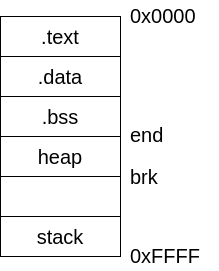
\includegraphics[width=150px]{images/25_Programmazione_C/memory_layout.png}
\end{figure}
otlre alle sezioni del file oggetto che abbiamo visto prima compaiono altre strutture:
\begin{itemize}
    \item heap: è la memoria dinamica allocata chiedendola al sistema operativo tramite alcune operazioni (malloc in C o new in C++ per esempio)
    \item stack: è la porzione di memoria relativa allo stack
    \item end: è un simbolo che indica la fine del programma
    \item brk: indica la fine della heap
\end{itemize}
inoltre c'è un altro simbolo \verb{start{ che indica l' entry point del programma, cioè la prima istruzione da eseguire.

Come si può notare tra la heap e lo stack c'è della memoria che non ha un nome, quella è memoria non inizializzata e può essere usata per allargare la heap o per allargare lo stack.
Lo stack viene allargato in automatico al primo accesso fuori dalla zona, la heap si allarga chiamando delle primitive esplicitamete.

\subsubsection{Differenze con AVR}
Questo layout e questi comportamenti non possono essere implementati anche sull' AVR, questo perché il codice ed i dati non sono nella stessa memoria, avendo due spazi di indirizzamento diversi, ed in più non abbiamo un sistema operativo che possa gestire questi allargamenti.

In AVR la memoria FLASH è indirizzata a singola riga, quindi una riga da due byte ha un indirizzo univoco, GCC invece ragiona a singoli byte quindi spesso gli indirizzi differiscono, sarà poi il linker a mettere tutto a posto.

\subsection{GCC toolchain}
La toolchain che si utilizza per usare il C sui uC si compone di diversi software che in genere sono tutti racchiusi in uno solo: \verb{gcc{ ed anche di librerie preconfezionate: le librerie standard.

\subsubsection{GCC}
La componente propriamente chiamata \verb{gcc{ è la componente compilatore.
Prende il nostro codice in C e produce la sua traduzione in codice assembly.

\subsubsection{GAS}
La componente \verb{GAS{ è il GNU assembler cioè l' assemblatore.
Prende il codice in assembly (sia che sia stato scritto da noi sia che sia frutto di una compilazione) e produce in uscita un file oggetto.

Partendo da diversi sorgenti posso produrre diversi file oggetto, ogni file oggetto avrà le proprie sezioni text, bss e data ed inizieranno tutte allo stesso indirizzo 0.

\subsubsection{Linkder - ld}
Il linker in fine si occupa di mettere tutti i file oggetto desiderati insieme e produrre il file ELF definitivo.
Si occupa di mergiare le varie sezioni con nomi uguali tutte assieme, aggiustare gli offset relativi e posizionare gli indirizzi laddove sono necessari da modificare.

Questo software vuole che gli si dica cosa fare con i file oggetto passati, va quindi specificato un \emph{linker script} che contiene gli indirizzi ai quali posizionare le varie sezioni per costruire le mappe di memoria che si vogliono.

Fortunatamente non dobbiamo scriverlo noi in quanto la toolchain che ne mette a disposizione vari per i vari microcontrollori quindi non ci basterà altro che specificare di star linkando del codice per un ATMEGA32.

\subsubsection{Librerie}
Una libreria è una collezione di codice scritto da altri e disponibile pronto all' utilizzo.
Per creare una libreria si scrivono le funzioni in file separati, si compilano, si assemblano ed i rispettivi file oggetto vengono inseriti in un archivio ottenuto con il comando \verb{ar{.
La convenzione è che questi archivi prendano il nome \verb{lib<name>.a{ ad esempio: \verb{libc.a{, \verb{libm.a{, \verb{libjpeg.a{.

\subsubsection{File crt}
Importanti sono inoltre i file C runtime: \verb{crt0.o{ è un file oggetto che contiene il codice iniziale da eseguire che poi va a chiamare il nostro codice.
Anche questo file va passato al linker e va passato come primo file in modo che in memoria si trovi ai primi indirizzi.

\subsection{Successo della toolchain}
Il C e tutto l' ecosistema ha avuto un grande successo perché un compilatore C si scrive in poco tempo perché non ha bisogno di funzioni operative, tutte le funzioni che abbiamo ed usiamo sono prese da una qualche libreria standard.
Per portare GCC da una architettura all' altra si deve quindi modificare solamente la libreria.

Ci permette inoltre di astrarre dall' hardware per certi versi:
\begin{verbatim}
    x = y / z;
\end{verbatim}
sarebbe una divisione, che sull' ATMEGA32 non si potrebbe fare, tuttavia la libreria obbligatoria \verb{libgcc.a{ implementa una funzioe per la divisione ed il compilatore traduce questa espressione in una chiamata a questa procedura.

\subsection{Esempio di programma in C}
Scriviamo un programma che esegue il blink di un led:
\begin{verbatim}
    #include <avr/io.h>
    #define TEMPO 10000
    
    void aspetta();
    
    int main(){
        DDRA = (1 << PINA0);
        while(1){
            PORTA |= (1 << PINA0);
            aspetta();
            PORTA &= ~(1 << PINA=);
            aspetta();
        }
        return 0;
    }
    
    void aspetta(){
        int i = 0;
        for(i=0; i < TEMPO; i++);
    }
    
\end{verbatim}
Per prima cosa si deve sempre importare la libreria \verb{avr/io.h{, assieme alla specifica del uC che stiamo usando permette di includere tutte le informazioni utili per questo microcontrollore.

Si noti che il modo con il quale facciamo aspettare il programma è uno dei peggiori possibili in quanto non sapendo come verrà tradotto non sappiamo quanto dura una singola iterazione, inoltre non sappiamo se le ottimizzazioni del compilatore lasceranno il ciclo lì o lo toglieranno per ottimizzare.
Un altro modo di fare questa attesa è quella di utilizzare le funzioni di libreria che implementano l' attesa attiva, oppure possiamo scrivere un sottoprogramma in assembly che sicuramente non verrà ottimizzato dal compilatore:
\begin{verbatim}
    .section text
    .global aspetta
    
    aspetta:
        push r24
        push r25
        ldi r24, lo8(20000)
        ldi r25, hi8(20000)
        
    1:
        sbiw r24, 1
        tst r24
        brne 1b
        tst r25
        brne 1b

        pop r25
        pop r24
        ret
\end{verbatim}
Specifichiamo che una volta assemblato questo codice deve essere localizzato nella sezione \verb{.text{ e che il simbolo \verb{aspetta{ deve poter essere visibile anche all' esterno del corrente file.

In fine si noti l' utilizzo delle etichette relative, le etichette composte da un singolo numero sono riutilizzabili e per saltarvi sopra si usano le direzioni:
\begin{itemize}
    \item \verb{1b{: saltare alla prima etichetta 1 che precede l' istruzione
    \item \verb{1f{: saltare alla prima etichetta 1 che segue l' istruzione
\end{itemize}

\subsection{Layout del file ELF}
Il layout del file ELF risultante è:
\begin{figure}[H]
    \centering
    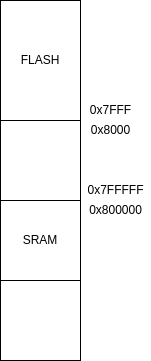
\includegraphics[width=100px]{images/25_Programmazione_C/ELF_layout.png}
\end{figure}
Si noti che sia la flash che la SRAM sono inserite nello stesso spazio di indirizzamento, questo perché il linker è in grado di produrre solo questo e non sa che AVR prevede due spazi di indirizzamento diversi.
Per risolvere questo problema il linker script pone la SRAM molto distante dalla fine della flash ed il programma che si occupa di caricare il programma sul uC taglierà gli indirizzi ai primi 2 byte, in questo modo tutto torna all' atto dell' esecuzione.

\subsection{Inizializzazione}
Come abbiamo già detto il programmatore si occupa di scrivere solamente la memoria FLASH, non la SRAM.
Quando però creiamo delle variabili globali esse finiranno nella sezione \verb{.data{ che in teoria dovrebbe finire nella RAM in quanto queste variabili possono variare.
Ma se programmiamo la RAM al prossimo riavvio del uC abbiamo perso i dati.

Per risolvere qusto problema la sezione \verb{.data{ viene inserita all' interno della FLASH ed allo startup del uC si copia in SRAM.
Il codice che si occupa di fare ciò è inserito direttamente dalla toolchain che si occupa di compilare, assemblare e linkare.

\subsubsection{.rodata}
In alcune situazioni potrebbe essere utile inserire delle variabili costanti nella FLASH in quanto evitiamo di utilizzare la SRAM per allocare informazioni che non cambieranno mai.
Per questi utilizzi possiamo creare la sezione \verb{.rodata{ (read-only data) che va in FLASH.
Il C normale non permette di utilizzare queste strutture perché non riesce a gestire due spazi di indirizzamento, dobbamo ricorrere a delle librerie esterne o ad altri compilatori.

\subsubsection{Doppi indirizzi per la .data}
Dal momento che poniamo la sezione \verb{.data{ è in FLASH prima di essere caricata in memoria il linker deve associare due indirizzi diversi alla stessa sezione.
L' indirizzo all' interno della FLASH è detto LMA, l' indirizzo all' interno della SRAM, quindi dopo la rilocazione, è detto VMA.

Ovviamente tutto il codice che deve accedere alle variabili accederà all' indirizzo VMA mentre il codice di inizializzazione che copia i valori dalla FLASH alla SRAM legge da LMA e scrive in VMA.

Si noti che la sezione \verb{.bss{ viene creata da un' altra subroutine che legge la dimensione ed alloca tanto spazio nella SRAM quanto ne serve.


\subsection{Esempio: sensore di parcheggio in C}
Vogliamo generare un' onda quadra a 40KHz con un burst di 10 periodi, possiamo quindi usare il timer 0.
\begin{verbatim}
    #include <avr/interrupt.h>
    // usato per includere le funzioni di utility
    // per gli interrupt
        
    void init_timer(){
        TCCR0 = (0 << COM01) | (1 << COM00) |
                (1 << WGM01) | (0 << WGM00);
        // modalità contatore con reset sul match,
        
        OCR0 = 12;
        // con clock ad 1 MHz ci bastano 25 clock
        // quindi 12 semiperiodi
        
        TIMSK |= (1 << OCIE0);
    }

    volatile int periodi;    
    void burst(){
        TCCR0 |= (1 << CS00);
        periodi = NPER*2;
    }

    // Macro utilizzata per inserire una interruzione
    // nel vettore di interruzioni
    ISR(TIMER0_COMP_vect){
        if(periodi <= 0)
            TCCR &= ~7;
            // Tolgo i bit CS

        periodi--;
    }
    
    void main(){
        init_timer();
        sei();
        // Abilita le interruzioni
    
        while(1){
            burst();
            while(periodi > 0);
        }
    }
\end{verbatim}
Si notino:
\begin{itemize}
    \item la variabile utilizzata nella interruzione è dichiarata \verb{volatile{ in quanto non deve essere oggetto di ottimizzazioni da parte del compilatore
    \item la funzione handler dell' interruzione del timer è dichiarata usando la macro \verb{ISR(TIMER0_COMP_vect){
\end{itemize}

\subsection{Leggere la memoria flash in C}
In assembly abbiamo delle istruzioni per leggere direttamente la flash (LPM), in C tuttavia no.
Se ho dei dati statici che non muteranno nel corso dell' evoluzione del programma copiarli in RAM è quantomeno inutile, a volte addirittura un problema, conviene collocarle in memoria flash e leggerla quando serve.

Possiamo istruire il compilatore di collocare alcuni dati in una sezione diversa da quella \verb{.data{ utilizzando:
\begin{verbatim}
    __attribute__((section(".sezione")))
        char stringa[] = "Manz";
\end{verbatim}
ed il linker di default è istruito per posizionare la sezione \verb{.progmem{ direttamente ed esclusivamente in flash, in definitiva:
\begin{verbatim}
    __attribute__((section(".progmem")))
        char stringa[] = "Manz";
\end{verbatim}

Tuttavia c'è un metodo molto più veloce che prevede l' utilizzo delle utility della libreria \verb{pgmspace.h{:
\begin{verbatim}
    PROGMEM char stringa[] = "Manz";
\end{verbatim}
oppure ancora, nel caso esplicito delle stringhe:
\begin{verbatim}
    char *s;
    s = PSTR("stringa che finirà in FLASH");
\end{verbatim}
fornisce l' indirizzo in FLASH nel quale si trova la stringa avendogli associato un simbolo randomico.

Per leggere un byte dalla flash ci sono varie funzioni di utilità:
\begin{verbatim}
    pgm_read_byte(address);
\end{verbatim}

\subsection{Puntatori}
\subsubsection{Utilizzo delle periferiche in C}
Abbiamo visto che per utilizzare delle periferiche ci basta usare i nomi dei loro registri ed il compilatore C farà tutta la magia.
Vedendo come traduce il preprocessore del C ci accorgiamo che l' istruzione:
\begin{verbatim}
    DDRA = (1 << PINA3);
\end{verbatim}
viene tradotta in:
\begin{verbatim}
    (*(volatile uint8_t *)((0x1A) + 0x20)) = (1 << 3);
\end{verbatim}
quindi ogni "costante" che riferisce un registro periferica viene trasformato in un accesso in memoria tramite puntatori esplicitamente riferiti con il loro indirizzo di memoria.

Da notare la somma tra 0x1A e 0x20 in quanto l' accesso alle periferiche è eseguito tramite istruzioni \verb{st{ ed \verb{ld{ e non tramite \verb{in{ e \verb{out{.

\subsubsection{Un po' di chiarezza}
Supponiamo di aver creato una variabile intera:
\begin{verbatim}
    int x = 0xabcd;
\end{verbatim}
oltre ai tipi di variabili "normali" esistono le variabili puntatori:
\begin{verbatim}
    int *px;
\end{verbatim}
Un puntatore è una variabile destinata a contenere numeri che sono indirizzi, in questo processore quindi sono variabili a 16 bit.

Per prendere un valore da dare a questo tipo di variabili si deve usare l' operatore \verb{&{ :
\begin{verbatim}
    px = &x;
\end{verbatim}
quindi ora la variabile \verb{px{ contiene l' indirizzo di \verb{x{.

Una volta che ho un puntatore alla variabile posso usarlo per eseguire un indirizzamento indiretto, in pratica posso scrivere nella variabile che sto puntando così come farei se usassi la variabile stessa:
\begin{verbatim}
    x = 17;
    *px = 17;
    // Fanno la stessa cosa!
\end{verbatim}

Posso ovviamente creare puntatori a puntatori:
\begin{verbatim}
    int q;
    int *pq = &q;
    int **ppq = &pq;
    
    q = 10;
    *pq = 10;
    **ppq = 10;
    // Fanno tutti la stessa cosa!
\end{verbatim}

\subsubsection{Regola aurea per leggere i tipi}
Dato un simbolo esso può essere seguito da:
\begin{itemize}
    \item \verb{[..]{: in questo caso si sta parlando di un array
    \item \verb{(..){: in questo caso si sta parlando di una funzione
\end{itemize}
\begin{verbatim}
    int a[10];
\end{verbatim}
$a$ è un array di interi.

\begin{verbatim}
    int f();
\end{verbatim}
$f$ è una funzione che ritorna un intero.

\emph{Partendo dal simbolo: vado a destra se si può, a sinistra se si deve!}
\begin{verbatim}
    int *a[4];
\end{verbatim}
partendo dal simbolo $a$, vado a destra, quindi $a$ è un array di 4 elementi.
Non posso andare più a destra perché è finito quidi vado a sinistra: $a$ è un array di puntatori ad intero.

\begin{verbatim}
    int (*a)[4];
\end{verbatim}
partendo dal simbolo $a$ non posso andare a destra perché devo eseguire le parentesi, quindi $a$ è un puntatore ad un array di interi (vado a sinistra).

\subsubsection{Puntatori a funzione}
\begin{verbatim}
    int *p(void);
\end{verbatim}
$p$ è una funzione che restituisce un puntatore ad intero.



